\makeatletter
\newcommand*{\compress}{\@minipagetrue}
\makeatother

\begin{figure}[h]
	\centering
	\missingfigure{Klassendiagramm}
	\caption{Klassendiagramm - A}
	\label{fig:klassendiagramm-a}
\end{figure}

\begin{figure}[h]
	\centering
	\begin{tabularx}{\textwidth}{p{.25\textwidth} | X}
		\rowcolor[HTML]{C0C0C0}
		\textbf{Klassenname} & \textbf{Aufgabe} \\
		User & \compress \begin{itemize}
			\item Speicherung der Nutzerdaten, sowie einer künstlichen Datenbank-ID
			\item Eine Flag, die den Adminstatus festlegt
			\item Listen von erstellten, einsehbaren und veränderbaren Kompositionen
		\end{itemize}\\
		\rowcolor[HTML]{E7E7E7}
		Composition & \compress \begin{itemize}
		  \item Speicherung einer künstlichen ID
			\item Speicherung der Kompositionen als Graphen, durch Speicherung der Knoten und Kanten
			\item Speicherung des Urhebers und der Nutzenden mit Zugriffs- bzw. Bearbeitungsrechten
			\item Konvertermethode, zum Erstellen eines detaillierten, versendbaren Objektes
			\item Konvertermethode, zum Erstellen eines reduzierten Objektes
			\item Methode zum Erstellen eines UserAuthorizations-Objektes um Nutzerrechte später einzusehen
		\end{itemize} \\
		CompositionNode & \compress \begin{itemize}
			\item Speicherung eines Dienstes, für dessen Verwendung im Kompositionsgraphen
			\item Konvertermethode, zum Erstellen eines detaillierten, versendbaren Objektes
			\item Referenz auf CompatibilityAnswer um Kompatibilität der verbundenen Dienste darzustellen
		\end{itemize} \\
		\rowcolor[HTML]{E7E7E7}
		CompositionEdge & \compress \begin{itemize}
			\item Speicherung einer gerichteten Kompositionskante als Paar von Kompositionsknoten
			\item Konvertermethode, zum Erstellen eines detaillierten, versendbaren Objektes
		\end{itemize} \\
		Service & \compress \begin{itemize}
			\item Speicherung der Diensteigenschaften
			\item Speicherung der zum Dienst gelisteten Tags
			\item Speicherung einer künstlichen ID
			\item Speicherung je einer Liste der passenden Ein- bzw. Ausgabeformate
		\end{itemize} \\
		\rowcolor[HTML]{E7E7E7}
		Format & \compress \begin{itemize}
			\item Speicherung von Name, Version und Kompatibilitätsgrad
		\end{itemize} \\
		Compatibility & \compress \begin{itemize}
			\item Utilklasse
			\item Methode zum bestimmen der Kompatibilität zweier Dienst
			\item Methode soll für Einzelanfragen und Kanten verwendet werden
		\end{itemize} \\
	\end{tabularx}
	\caption{Klassen des Models}
	\label{table:klassenbeschreibung-a}
\end{figure}

\begin{figure}[h]
	\begin{tabularx}{\textwidth}{p{.25\textwidth} | X}
		\rowcolor[HTML]{C0C0C0}
		\textbf{Klassenname} & \textbf{Aufgabe} \\
		DetailComp & \compress \begin{itemize}
			\item Erbt von SimpleComp und speichert damit Metadaten zur Komposition (ob bearbeitbar, Name und ID)
			\item Listen der User (als SimpleUser) mit Bearbeitungs- bzw Einsichtrecht
			\item Verweis auf Autor
		\end{itemize}\\
		\rowcolor[HTML]{E7E7E7}
		Edge & \compress \begin{itemize}
		  \item Besteht aus einem geordneten Paar von Nodeobjekten, dem Eingang- und Ausgangsknoten.
			\item Speicherung der Kompatibilität der Dienste anhand einer CompatibilityAnswer
		\end{itemize}\\
		Node & \compress \begin{itemize}
			\item Speicherung der Position und Verweis auf den verwendeten Service
		\end{itemize}\\
		\rowcolor[HTML]{E7E7E7}
		SimpleComp & \compress \begin{itemize}
			\item Speicherung der elementarsten Daten für die Listenansicht der Komposition
		\end{itemize}\\
		SimpleUser  & \compress \begin{itemize}
			\item Speicherung der elementarsten Daten (ID und Name)
		\end{itemize}\\
		\rowcolor[HTML]{E7E7E7}
		DetailUser & \compress \begin{itemize}
			\item Erbt von SimpleUser
			\item Dient der Bearbeitung der User
			\item Flag um User als Administratoren zu markieren
			\item Keine Passwortvermerk
		\end{itemize}\\
		Alternative & \compress \begin{itemize}
			\item Speicherung der möglichen Konverter eventuell Konverterketten (Name, Versionsnummer, ID) um Kompatibilität zu erzeugen
		\end{itemize}\\
		\rowcolor[HTML]{E7E7E7}
		CompatibillityAnswer & \compress \begin{itemize}
			\item Speicherung der Kompatibilität zwischen zwei Diensten
			\item Speicherung der effektiv kompatiblen Formate
			\item Liste von Alternativen
			\item Zum Antworten auf Einzelanfragen zur Kompatibilitätsprüfung zweier Dienste
		\end{itemize}\\
		UserAuthorizations & \compress \begin{itemize}
			\item Speicherung je einer Liste für User mit Einsichts- bzw. Bearbeitungsrecht
		\end{itemize}\\
	\end{tabularx}
	\caption{Klassen des Models \textit{Fortsetzung}}
\end{figure}



\begin{figure}[h]
	\centering
	\missingfigure{Klassenbeschreibung Controller}
	\caption{Klassendiagramm des Controllers}
	\label{fig:klassendiagramm-a}
\end{figure}

\begin{figure}[h]
	\begin{tabularx}{\textwidth}{p{.25\textwidth} | X}
		\rowcolor[HTML]{C0C0C0}
		\textbf{Klassenname} & \textbf{Aufgabe} \\
		CompositionController & \begin{itemize}
		\item Klasse stellt einen REST-Controller dar
		\item Verschiedene Methoden zum Erstellen, Anfragen und bearbeiten von Compositions aus der Datenbank
		\item die Authorisierung des Nutzers wird in der Behandlung der Anfragen berücksichtigt
		\item Rückgabetyp ist stets ResponseEntity, da so ein entsprechender HTTP-Code als Antwort gegeben werden kann.
		\end{itemize}\\
		\rowcolor[HTML]{E7E7E7}
		ServiceController & \begin{itemize}
			\item Rest-Controller, analog zu CompositionController
			\item Verwaltet den Zugriff und Bearbeitung von Servicen.
		\end{itemize}\\
		UserController & \begin{itemize}
			\item REST-Controller, analog zu den anderen Klassen
			\item Erlaubt es Daten von User zu verändern
		\end{itemize}\\
		\rowcolor[HTML]{E7E7E7}
		UserPermission & \begin{itemize}
			\item REST-Controller
			\item Erlaubt es dem Owner einer Komposition die Zugriffsrechte auf selbige zu verändern.
		\end{itemize}
	\end{tabularx}
	\caption{Klassen des Models \textit{Fortsetzung}}
\end{figure}

\begin{tcolorbox}
Teilt eure Klassendiagramme bitte auf und baut \textbf{kein} einzelnes riesiges Diagramm.
Getter und Setter Methoden müssen hier nicht modelliert werden.
Sie sollten aber der klassischen Namenskonvention folgen, um die Nutzung in Sequenzdiagrammen zu ermöglichen.
\\\\
Auf jedes Diagramm folgt eine Tabelle, in der die Aufgabe \textbf{jeder} Klasse beschrieben wird.
\end{tcolorbox}

\section*{Klassendiagramm zur Android-App}

\begin{figure}[h]
	\centering
	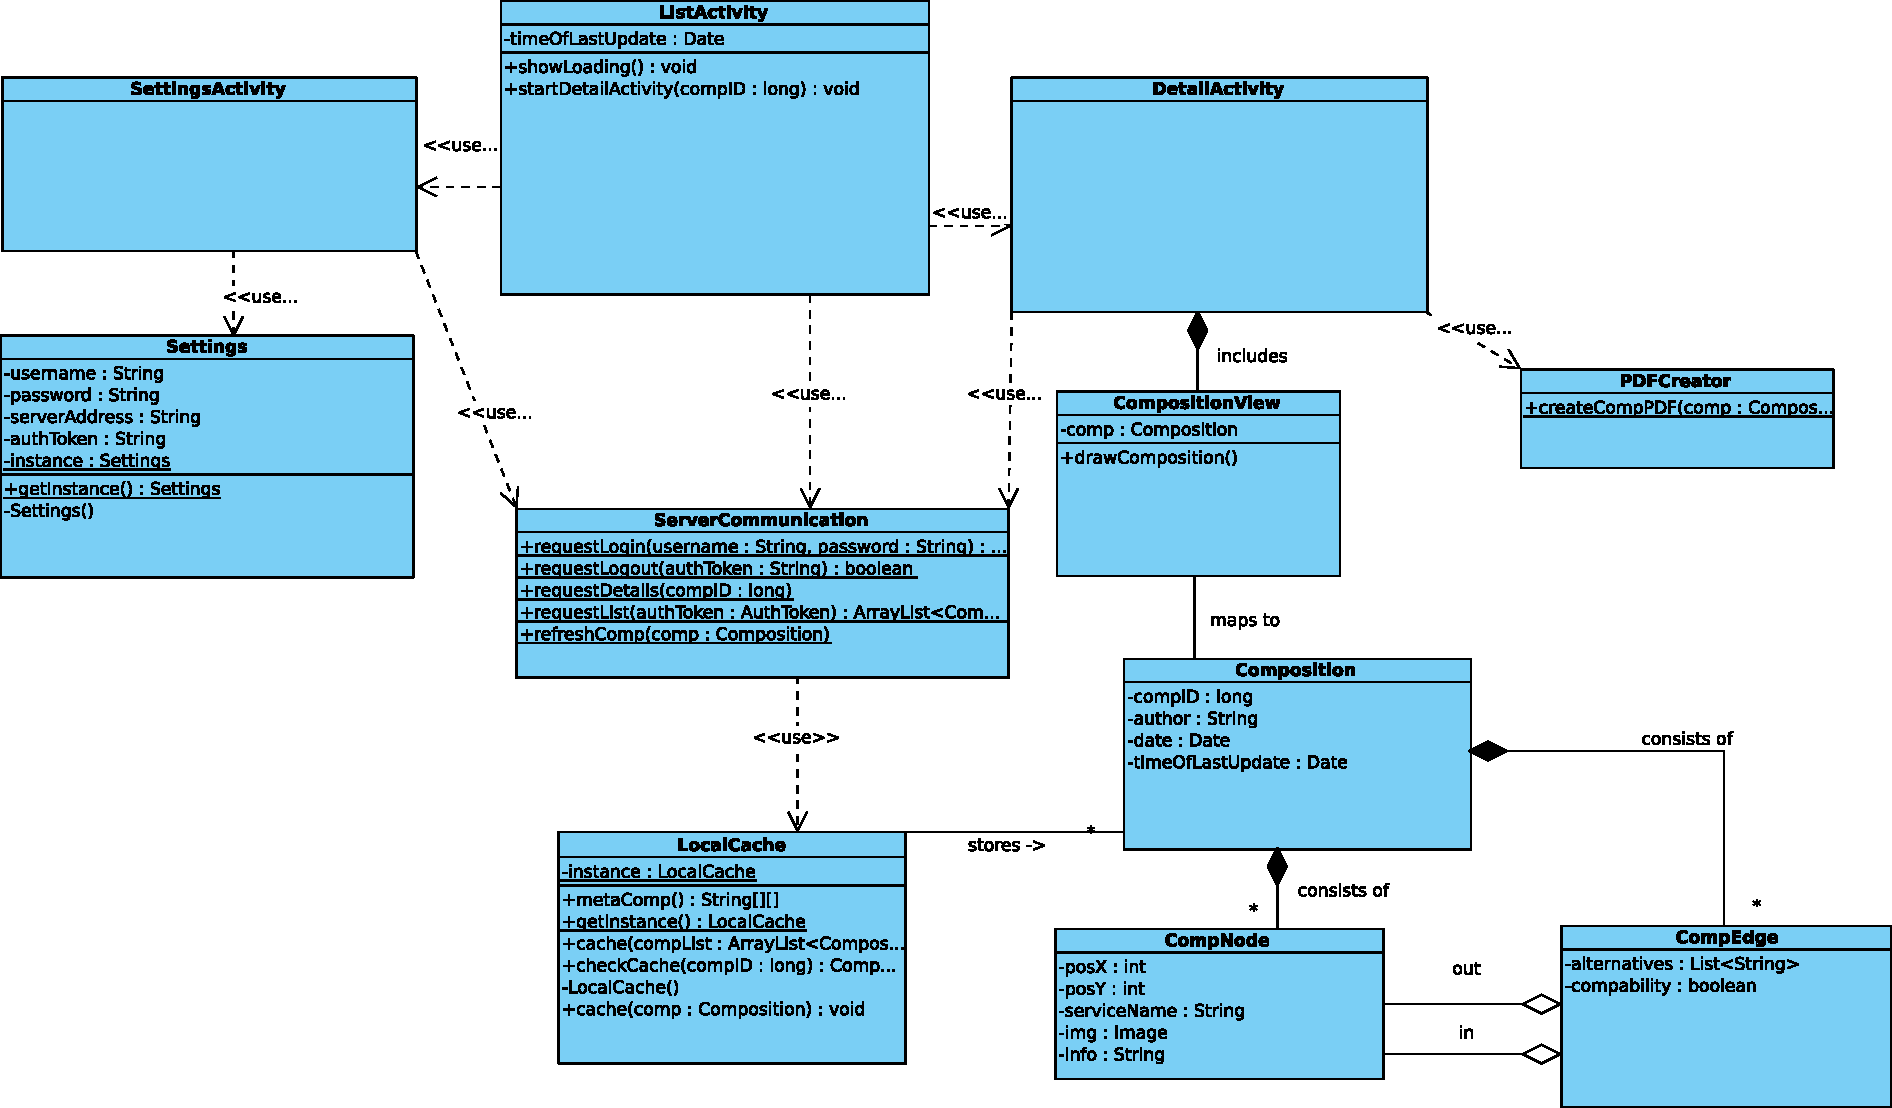
\includegraphics[width=\textwidth]{Klassendiagramm_App/Class_Diagram1}
	\caption{Klassendiagramm - App}
	\label{fig:klassendiagramm-a}
\end{figure}

\begin{table}[h]
	\centering
	\begin{tabularx}{\textwidth}{p{.25\textwidth} X}
		\rowcolor[HTML]{C0C0C0} 
		\textbf{Klassenname} & \textbf{Aufgabe} \\
		ListActivity & MainActivity und Übersicht über sichtbare Kompositionen  \\
		\rowcolor[HTML]{E7E7E7} 
		SettingsActivity & Activity zum Festlegen von Einstellungen, zum Einloggen und Festlegen der Serveradresse \\
		DetailActivity & Detailansicht zur grafischen Darstellung einer Komposition \\
		\rowcolor[HTML]{E7E7E7} 
		Settings & Dient zur Kapselung der getroffenen Einstellungen \\
		CompositionView & Eigentliche View, in der das Zeichnen einer Komposition stattfindet. Jede DetailActivity verfügt über ein CompositionView. \\
		\rowcolor[HTML]{E7E7E7} 
		Composition & Interne Model-Abstraktion einer Komposition \\
		CompNode & Interne Model-Abstraktion eines Diensts, der als Knoten in einer Komposition fungiert. \\
		\rowcolor[HTML]{E7E7E7} 
		CompEdge & Interne Model-Abstraktion einer Kante zwischen zwei Diensten in einer Komposition \\
		PDFCreator & Helper-Klasse zur Generierung von PDFs, die Kompositionsbilder beinhalten. \\
			\rowcolor[HTML]{E7E7E7} 
		ServerCommunication & Anlaufpunkt für sämtliche Kommunikation mit dem Backend: ServerCommunication übernimmt daraufhin die Aufgabe, Verbindungen zum Server herzustellen, die Daten zu interpretieren und im richtigen Format weiterzugeben. \\
		LocalCache & Cache zur Speicherung von durch Anfragen erhaltenden Daten, damit diese nicht erneut angefragt werden müssen. 
	\end{tabularx}
	\caption{Klassenbeschreibung - App}
	\label{table:klassenbeschreibung-a}
\end{table}